\documentclass[paper=a4, fontsize=11pt]{scrartcl}
\usepackage{fourier} 
\usepackage[portuguese]{babel}
\usepackage[utf8]{inputenc}
\usepackage{amsmath,amsfonts,amsthm,amssymb}
\usepackage{lipsum} 
\usepackage{sectsty}
\usepackage{graphicx}
\usepackage{amsmath,bm,bbm} 
\allsectionsfont{\normalfont\scshape}
\numberwithin{equation}{section} 
\numberwithin{figure}{section}
\numberwithin{table}{section} 
\newcommand{\horrule}[1]{\rule{\linewidth}{#1}} 

\begin{document}

\normalfont \normalsize 
\hspace{2.3cm} \textsc{universidade federal de alagoas -- Eduarda Chagas}\\[25pt]
\horrule{0.5pt} \\[0.5cm]
\huge Análise dos algoritmos de imputação de dados \\ 
\horrule{2pt} \\[0.5cm]
\normalfont \normalsize 

\section{Introdução}

Ao introduzir o conceito de entropia de permutação e o método de simbolização, Bandt e Pompe assumiram como condição inicial que os dados analisados consistiam de valores contínuos, possuindo assim uma probabilidade quase nula da existência de valores repetidos nas séries temporais analisadas, e nos raros eventos que a exceção ocorria, o recomendado era ignorar estes valores ou adicionar uma pequena pertubação. Entretanto, ao trabalhar com análise não-paramétrica de séries temporais discretas percebemos que tal fato ocorre com grande frequência devido a dois motivos: As séries podem ser produzidas por geradores discretos de dados ou serem discretizados como consequência da falta de precisão do dispositivo de medição de dados. Logo, algumas mudanças devem ser realizadas ao trabalhar com tais tipos de dados, uma das alternativas presentes na literatura, por exemplo, sugere modificar a estimação da Entropia de Permutação. Outra alternativa consiste em utilizar novas técnicas de simbolização dos padrões de Bandt e Pompe. 

O objetivo deste relatório é comparar as diferentes algoritmos de imputação de dados repetidos, considerando as duas estratégias possíveis (eliminar as observações com dados repetidos ou substituí-los por valores adequados) e analisando o seu comportamento no plano Entropia-Complexidade.

\section{Algoritmos de imputação de dados}

Ao partir da premissa de que as séries temporais estudadas foram obtidas por meio de geradores de dados contínuos e que os valores repetidos encontrados consistem em dados perdidos derivados de uma observação errônea do mundo real, existe vários métodos de manipulação dessas observações para realizar a análise desses dados.

\subsection{Complete Case}

Consiste no método proposto originalmente por Bandt e Pompe, onde elimina do cálculo da probabilidade todos os padrões formados por elementos repetidos. 

\subsection{Time Ordered Imputation} 

Uma das técnicas mais utilizadas na lituratura. Aqui a seguinte regra é seguida: se $x_{t1} = x_{t2}$ e $t_{1} < t_{2}$ então $x_{t1} < x_{t2}$.

\subsection{Random Imputation}

Nesta técnica é seguida a sugestão de Bandt e Pompe, onde eles recomendam quebrar numericamente as igualdades adicionando pequenas perturbações, devendo ser a amplitude desta perturbação menor que a diferença mínima entre dois valores diferentes no padrão. Random Imputation sugere que padrões com valores iguais são o resultado de uma observação grosseira de padrões sem repetições originalmente, logo eles devem ser mapeados em símbolos correspondentes aos padrões originais com o mesmo peso probabilístico. Desse modo, pesos são adicionados aos padrões, sendo $\omega = 1$ para os padrões sem elementos repetidos e $\omega = 1/n$, onde $n$ determina o número de possíveis padrões, dado um determinado conjunto de elementos contendo valores repetidos. Assim, a probabilidade dos padrões resultantes será calculada considerando tais pesos.

\subsection{Data Driven Imputation}

O método de imputação Data Driven (DDMI) consiste de uma metodologia semelhante ao Random Imputation mas, ao invés de adicionar uma perturbação aleatória com igual probabilidade para cada símbolo adequado, estas probabilidades são originadas de uma PDF previamente conhecida calculada por meio do método Complete Case.

\section{Simulação numérica}

Nesta secção, os algoritmos citados acima, Complete Case, Time Ordered, Random Imputation e Data Driven Imputation são avaliados usando dados de processos caóticos simulados. Para obter um conjunto reproduzível de séries temporais, os mapas logísticos foram simulados usando os seguintes valores:

\begin{itemize}
    \item Condição inicial: $X_{0} = 0.1$
    \item Valor do parâmetro: $r = 4$
\end{itemize}

A simulação consistiu do estudo de 100 séries obtidas por meio da iteração do mapa logístico com as características citadas acima, onde cada série possui comprimento $N = 30.000$ e foram obtidas por meio de interações sequenciais do mapa. Os primeiros $10^3$ valores do mapa logístico foram descartados do estudo.

Todas essas séries não apresentam valores repetidos e tais dados serão referidos como a \textbf{série temporal original}. Depois disso, foi criado um método de ataque para as séries temporais. Para cada série geramos uma amostra aleatória de mesmo comprimento seguindo a distribuição de Bernoulli, onde por meio desta verificamos se um dado será ou não atacado. Cada dado atacado perderá o seu valor original e receberá o valor do elemento que o antecede criando assim valores repetidos ao longo da série temporal, levando a uma versão grosseira dessas séries temporais originais.

Após a geração das séries temporais e realizado o ataque dos dados, foram calculados os valores da Entropia normalizada de Shannon e a medida de Complexidade estatística generalizada, onde para as séries atacadas foram utilizados os quatro algoritmos de imputação apresentados e para as séries originais foi seguido o algoritmo tradicional de simbolização de Bandt e Pompe.  Para a simbolização utilizamos como parâmetros dimensão $D = 6$ e delay $\tau = 1$.

\section{Resultados e conclusões}

A Fig.~\ref{fig:Plano} nos mostra o comportamento no plano $(H(\bm h), C(\bm h, \bm u))$ das séries originais e das séries atacadas utilizando os diferentes algoritmos de imputação para $D = 6$ e $\tau = 1$.

\begin{figure}[hbt]
	\centering
	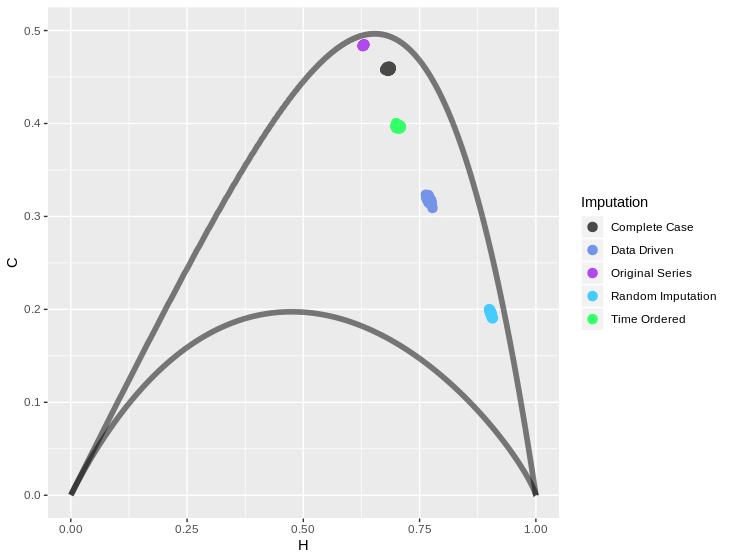
\includegraphics[scale = 0.6]{hcplane.png}        
     \caption{Plano Entropia-Complexidade das séries geradas.}
     \label{fig:Plano}
\end{figure}

O Plano $(H(\bm h), C(\bm h, \bm u))$ se mostra uma eficiente ferramenta de distinção entre a natureza caótica e estocástica de séries temporais, uma vez que os quantificadores de permutação possuem comportamentos distintos para diferentes tipos de dinâmica. Como já se é conhecido, mapas caóticos possuem como comportamento típico valores de entropia $H(\bm h)$ intermediários, enquanto a complexidade $C(\bm h, \bm u)$ atinge valores maiores, próximos ao limite $C_{max}$. Além disso, comportamento semelhante ainda é observado quando as séries temporais dos mapas caóticos estão contaminadas.

Como podemos verificar a metodologia do Random Imputation superestima a entropia ao adicionar ruído aleatório à série com o objetivo de quebrar as igualdades. As demais metodologias, Time Ordered e Data Driven se mostram ser bons estimadores, uma vez que são mais precisos que simplesmente eliminar os padrões com relação à perda de informação que isso representa.


\end{document}